\section{Human aware Navigation Model}
\label{social_nav}



\begin{figure}
\centering
{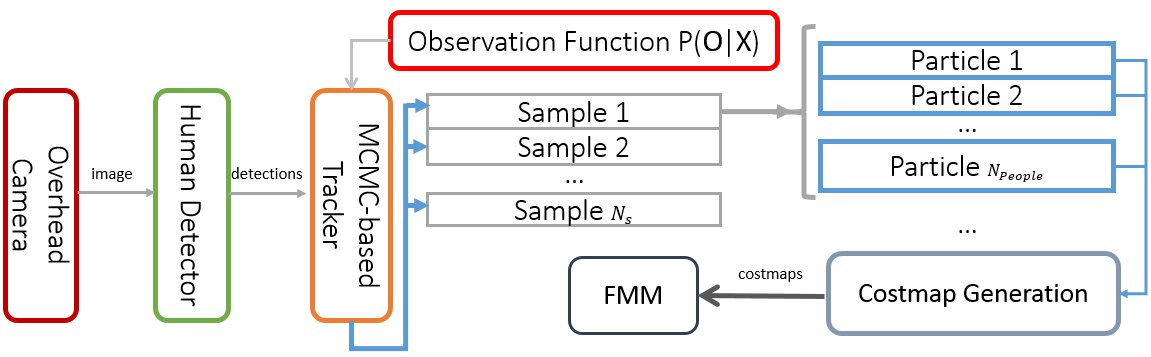
\includegraphics[width=0.49\textwidth]{pictures/block.jpg}}
\caption{System components diagram.}
\label{fig:block}
\end{figure}

%\dv{Sections 3 and 4 can be used to explain our model. First the perception and then the human aware navigation model. Don't spend too much time explaining the background of these methods. Make that brief and explain more on our approaches. It is a bit confusing when you split social path planning and navigation. I feel its better to have it under the same section. We have one Human aware navigation model which could have a subsection for social cost and such and another for navigation(FMM,DWA).}

In this section we will explain the navigation component of the system and describe the social cost computations methods that provide the information required for our socially-aware FMM-based path planner. Fig. \ref{fig:block} shows the system components and their connections.

%The model used for achieving human-aware navigation, mainly consists of accounting for social costs in the planners. In this work we focus on modelling social costs based on the proxemics principle, targeted for real robotic applications in the presence of noisy perception. These costs are then used in an FMM-based global planner, resulting in trajectories that respect social considerations.% However, we extend the deterministic model of social costmaps, for taking the uncertainty of perception into account. For this purpose, three different methods have been proposed in combination with a probabilistic tracker, for obtaining uncertainty-based social costs. 

%Our goal is to show that the assumption of having perfect information about the state of the human is unrealistic and in real situations when the robot has to deal with uncontrolled environments, the uncertainty in this information can not be ignored. We can think of false negative detections where the robot misses to take an person into consideration, false positive detections where other objects are detected as humans, noisy estimations of position, orientation, velocity of the person, etc. %To the best of our knowledge, there does not exit any work on including uncertainty of perception in the social costs model.

\subsection{Navigation Framework}

The robot navigation is based on the navigation system used in the MOnarCH project~\cite{monarch2013}, detailed in~\cite{ventura2015}. As input, it uses the pose estimates provided by a standard AMCL self-localization system~\cite{amcl}, given odometry, laser range finder readings, and a static map. The navigation system is based on FMM for motion planning, together with a Dynamic Window Approach (DWA) algorithm for guidance and obstacle avoidance~\cite{fox1997dynamic}. DWA is essentially a maximization (over a discrete set of feasible velocity candidate commands) of an evaluation function translating three guidance goals: (1)~progress towards the goal, (2)~clearance from obstacles, and (3)~absolute speed.

The potential field output by FMM is minima free and yields an optimal path from a given initial to a final goal point. It is optimal in the sense that the integral of a costmap over the path is minimal, given the initial and final points as boundary conditions.
% The path is the solution of a gradient descend Ordinary Differential Equation (ODE), with the initial point as initial condition.
However, we do not explicitly compute a path. Instead, we compute the progress towards the goal directly from the gradient of the potential field. FMM has been used in MOnarCH before, considering solely an increased cost near static map obstacles in its costmap. This keeps the resulting paths away from the obstacles. In this paper a \emph{social} component is added to this costmap as well.% This social costmap is explained in the next section.

FMM and DWA run asynchronously. FMM is activated when either a new goal position is given, or when the costmap changes, and DWA is running in a closed loop with a fixed rate% of 20 \textit{Hz} in our experiments
, using the last updated potential field from the FMM.

%Navigation in this context is understood as the capability of a robot to move autonomously in the environment with the goal of reaching a pre-specified final pose. The time taken by the robot to execute this task should be minimal, while avoiding collisions with obstacles as well as maintaining a certain clearance to them. In this paper we take the classical approach of dividing navigation into self-localization and guidance, assuming knowledge of a map of the environment. We also assume that unmapped static or moving obstacles may appear in the environment, while the robot is expected to deal with them in an appropriate way. We further assume an existing self-localization system (AMCL \cite{amcl}), based on data fusion of odometry and range sensor matching with the map. 

%The guidance problem is approached as a two step process. First, given a goal location, the robot plans its path from the current pose to the goal pose. This is the task of our FMM-based global planner. Second, the plan is executed by the robot, in real time, while avoiding unmapped obstacles. This is done by means of a local path planner based on DWA \cite{fox1997dynamic}. More details on the navigation can be found in \cite{ventura2015}.

\subsection{Social Costs}


%\dv{rewrite this in a way that we dont model orientation, but people do that too and its a possible but not mandatory part of our work.}
The personal space around a human can be defined as the mixture of two pseudo-Gaussian functions, one for the front and another one for the rear part of the area surrounding the person. The orientation and heading of the person will cause a corresponding rotation in these functions in such a way that the person is always in the center and the absolute orientation of the person matches that of the Gaussian functions. 
A Gaussian function $\phi$, centered on $p$ with covariance matrix $\Sigma$, is defined as follows:

\begin{equation}
\phi(q) = exp\begin{Bmatrix}
-\frac{1}{2}(q-p)\Sigma^{-1}(q-p)
\end{Bmatrix}\end{equation}
$q$ indicates the position of a point and $\Sigma$ is:
\begin{equation}
%\scriptsize 
\Sigma = \begin{pmatrix}
{\sigma}_{x}^2  & 0\\ 
 0& {\sigma}_{y}^2 
\end{pmatrix}
\end{equation}
${\sigma}_{x}$ and ${\sigma}_{y}$ are used to modulate the shape of the Gaussian and are traditionally chosen in a way to respect the personal space of a person as indicated by the proxemics principle. Various factors can influence the size of this area, however ${\sigma}_{x}$ and ${\sigma}_{y}$ are commonly considered to be constant. Getting closer to a person, will cause an increase in the value of this function, and hence the social cost associated to that position will increase.

If the center of the costmap, which indicates the position of the person is not deterministically known, the costmap can not correctly model the social costs and hence the social path planning could fail in finding an appropriate socially compliant path. This problem becomes much more critical in real applications where robustness is vital for succeeding under different conditions. We believe probabilistic social costs can be a remedy to this problem. 


In the following, we will go into the details of computing social costs with the particles obtained from the MCMC-based tracker. Using the concept of layered costmaps similar to \cite{lu2014iros}, an FMM planner uses this information for performing the replanning.% It should be emphasized that the proposed methods are planner-independent and applicable as far as the costmap concept is supported. 
%FMM computes the optimal path for the robot for a given destination, according to a potential filed created by the setting of obstacles in an environment based on wave propagation principles. In our system, social costs are incorporated into the FMM method when computing the optimal path by means of imposing them as virtual obstacles.
\subsubsection{Uncertainty-based Social Costs}

%To include the uncertainty of perception in our model, we need to have an estimate of the underlying distribution of people present in the environment at each time step. This is given by the MCMC-based tracker, that 
The MCMC-based tracker provides samples of the \textit{union} of the probability distributions for having a person in a given environment. More specifically, a predefined number of joint samples are reported at each time step, containing a set of particles for each person that the tracker detects. In the following, we propose two types of methods for using the particles given by these samples, to create social costmaps.  


\subsubsection*{\normalfont \textbf{Convolution}}

The core idea we propose for incorporating uncertainty in the costmap is to compute an \textit{expectation} based costmap.
%In other words, we treat the probability map of the presence of people in the environment as a two dimensional signal and convolve it with the conventional Gaussian costmap, to obtain the final probabilistic social costs. 
%If $K$ is a 2D Gaussian kernel of size $m\times n$ representing the social costmap, the social cost of each grid cell is computed as follows:   
%\begin{equation}
%Costs (i,j) = \sum_{k=1}^{m}\sum_{l=1}^{n}ProbabilityMap(i
%+k-1, j+l-1)K(k,l)
%\end{equation}
 Consider a person at $(x_{p},y_{p})$, the deterministic costmap at $(x,y)$ is:
\begin{equation}
    C(x, y;x_{p}, y_{p}) = K(x-x_{p}, y-y_{p})
\end{equation}
$K$ is the 2D Gaussian, modeling the standard social costmaps, \textit{i.e.}, it is $\phi$ when $q=\begin{bmatrix}
x\\ 
y
\end{bmatrix}$ and $p=\begin{bmatrix}
x_{p}\\ 
y_{p}
\end{bmatrix}$. The probabilistic costmap is given by the expected value of the cost $C$, given the person probability distribution $p(x_{p},y_{p})$:


\begin{multline}
 $ EC(x, y) = E_{p(x_{p}, y_{p})}[C(x, y;x_{p}, y_{p})] =\\ 
\int\int K(x-x_{p}, y-y_{p}) p(x_{p}, y_{p}) dx_{p}dy_{p}$
\end{multline}
This is a convolution. We approximate this expectation using a grid of probabilities $P$, obtained from the tracker particles:

\begin{equation}
   EC(i, j) \simeq \sum_{k}\sum_{l}K(i-k,j-l)P(k,l)
\end{equation}
By convolving all the particles from the MCMC tracker with the social costmap, we compute an \textit{expected costmap} incorporating all the uncertainty in the environment. This is a principled approach to solve the problem 
since we are not abstracting away any information provided by the perception system, and hence, in theory this approach should provide us with a costmap model that would be most informative for uncertainty-based human-aware navigation.

%We can compute the convolution of the estimate of the underlying distribution for the presence of people in an environment, by the conventional social costmap to get the final social cost for each position of the map.


%There are two main steps required for acquiring the final costmap of the environment using this approach. 1) Create a probability map for the presence of people in the environment, 2) by convolving this probability map with the Gaussian-shaped social costmap for an individual person, obtain the final social costmap that contains the social costs related to all the people present in the environment.
   
By taking this approach, the conventional 2D Gaussian shape of the social costmap is no longer mandatory, thus this costmap model is more flexible. Additionally, there is no need to know the number of people ahead of time as the particles given by tracker are reflecting this (refer to \ref{MCMC}).% \dv{add a picture somewhere of how the cost map looks}


\subsubsection*{\normalfont \textbf{Clustering}}
Another approach we propose is to abstract the uncertainty information in the samples by clustering the particles and then computing the uncertainty based on the features of the cluster. Upon receiving the position particles from the tracker we compute the center of the social costmaps, and the ${\sigma}$ values for all the people present in the environment. By clustering the particles and finding the centroids of the clusters, along with an uncertainty measure based on the spatial cluster scatter, we can adaptively compute the social costmaps at each time step. We will briefly describe the two clustering methods selected for our work in the following.
\paragraph{K-means clustering}

K-means clustering \cite{hartigan1979algorithm} method can be adopted for computing the costmap centers and $\Sigma$. However, one requirement for using this method is knowing K which is the number of clusters and in our case the number of people, ahead of time. This is not a realistic assumption for dynamic environments with multiple people. Nonetheless, we will test this method as a baseline for comparing the performances of other human-aware navigation methods.% both in simulation and reality.

\paragraph{Mean shift clustering}
To overcome the limitation of K-means clustering method for needing to know the number of clusters ahead of time, we chose another clustering method, mean shift clustering \cite{comaniciu2002mean}, that is able to determine the number of clusters given the particle set automatically. We used the median of all pairwise distances to estimate the bandwidth of the mean shift method.


\subsubsection{Deterministic Social Costs}
For the purpose of creating a baseline to compare our proposed model, we have also designed a deterministic model for the social costmap. 
Here, we use a deterministic output from the tracker, without considering the particles, by just using the mode of the distribution as deterministic location of the people, along with the conventional costmap model. 


This is the standard approach that is being used for social path planning in human-aware navigation, where it is assumed that the position and orientation of the person is deterministically known at every time step with no model of uncertainty. Once this information is known, the Gaussian-shaped costmap can be used to obtain the social costs. This costmap can be tuned according to the desired parameters. In this paper, we have taken an approach similar to \cite{gomez2013social} with ${\sigma}_{x} = 0.255\ m$, for deterministic costmaps. 


 

%In this paper, we focus on the social costmaps based solely on the position of the persons present in the environment. For deterministic social costs, this information is given by a deterministic tracker \dv{havent explained det. tracker} at each time step, and upon receiving this information the social costmap layer is updated. This approach is easily scalable for including multiple people.


%$P$ is a discrete map representation of a given resolution, containing the probability of each cell being occupied by a person.